\section{Adding new algorithms}

\subsection{Basic Structure}
\begin{itemize}
	\item Any algorithm used with VNREAL must be derived from MuLaViTo's \texttt{mulavito. IAlgorithm} interface which
	\begin{itemize}
		\item defines a common way to access status information of a running algorithm
		\item allows to show a GUI progress bar
	\end{itemize}
	\item The package \textit{vnreal.algorithms} contains several base classes (implementing \texttt{mulavito. IAlgorithm}) to derive own algorithms from
\item \texttt{vnreal.algorithms.AbstractAlgorithm} (shown left in figure \ref{fig:abstractAlgorithms}) merely provides abstract methods for doing stuff before and after running the algorithm 
\item \texttt{vnreal.algorithms.AbstractSequentialAlgorithm} (shown right in figure \ref{fig:abstractAlgorithms}) performs a sequential processing providing abstract methods \textsl{hasNext} and \textsl{getNext}
\begin{figure}[h]
  \begin{center}
		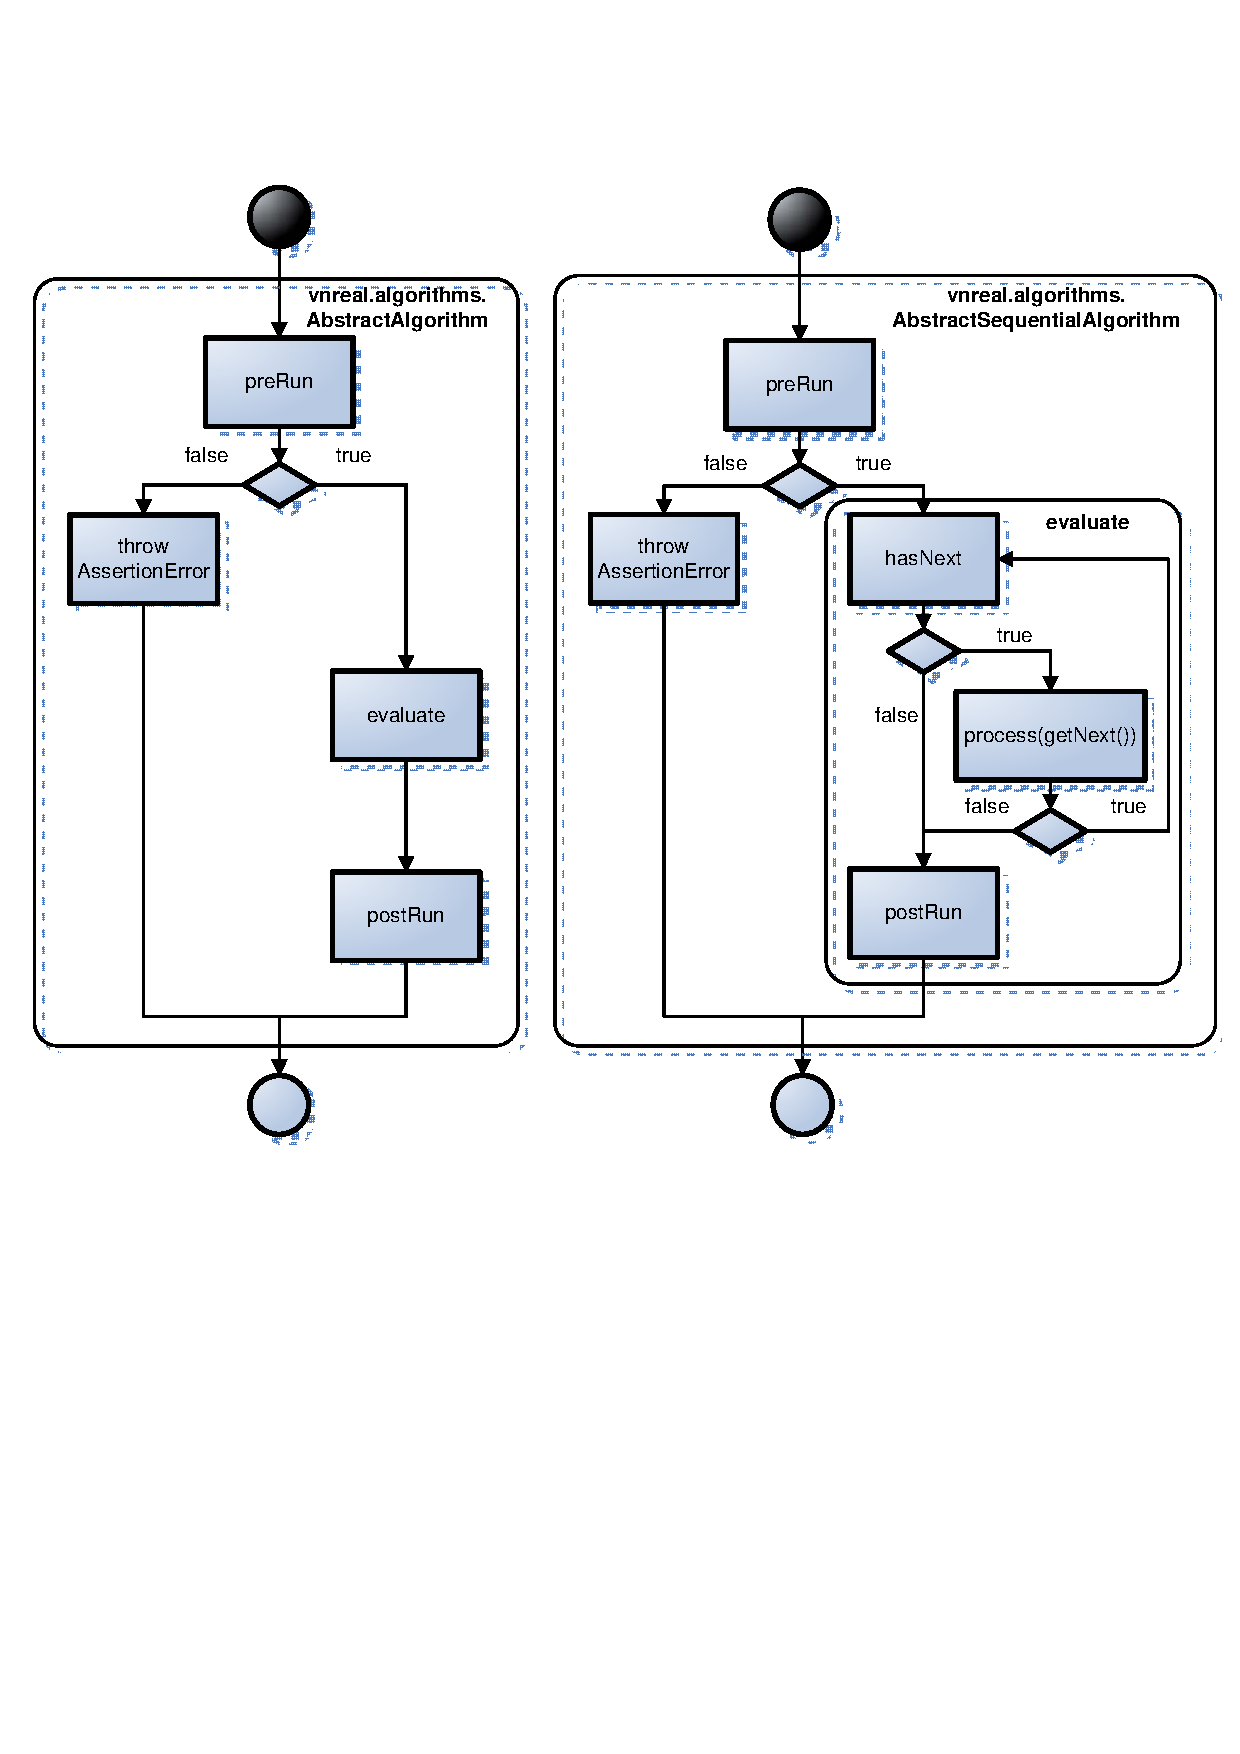
\includegraphics[width=\textwidth]{img/abstractAlgorithms.pdf}
	\end{center}
	\caption{Behaviour of \texttt{AbstractAlgorithm} and \texttt{AbstractSquentialAlgorithm} }
	\label{fig:abstractAlgorithms}
\end{figure}
\item \texttt{vnreal.algorithms.AbstractRevokableSequentialAlgorithm} additionally provides an abstract \textsl{revoke} method
\item Basic algorithmic principle
\begin{enumerate}
	\item The algorithm gets a \texttt{vnreal.network.NetworkStack} which consists of
	\begin{itemize}
		\item a \texttt{vnreal.network.substrate.SubstrateNetwork} with resources
		\item a list of \texttt{vnreal.network.virtual.VirtualNetwork} with demands
	\end{itemize}
	\item The algorithm performs the VNM and VLM by search for resources that are able to fulfill the given demands
\end{enumerate}
\end{itemize}



\subsection{Example}
The package \textit{vnreal.algorithms.samples} contains experimental algorithms, like the \texttt{Simple\-Dijkstra\-Algorithm}. This exemplary algorithm performs
\begin{itemize}
	\item an arbitrary virtual node mapping (choosing the node mapping in an arbitrary way among the substrate nodes accomplishing the virtual node demands), 
	\item the virtual link mapping is implemented by connecting each pair of mapped virtual nodes by the shortest path in the substrate network calculated using the Dijkstra algorithm.
\end{itemize}
The first part of the class \texttt{SimpleDijkstraAlgorithm} implementation looks like
\begin{lstlisting}
public final class SimpleDijkstraAlgorithm extends AbstractSequentialAlgorithm<VirtualLink> {
	private final NetworkStack stack;//Set of networks including the substrate network and the set of virtual network requests.
	private Iterator<? extends Network<?, ?, ?>> curNetIt;//Iterator over the set of virtual network requests
	private Iterator<VirtualLink> curIt;//Interator over the set of virtual links of a virtual network request 
\end{lstlisting}
This is the \textsl{hasNext} function of this algorithm which simply updates the iterator over the set of virtual network requests. If one virtual network requesthas already been served, it moves the \textsl{curNetIt} to the next virtual network request and updates \textsl{curNetIt} iterator. If there is no more virtual network requests it returns false. 
\begin{lstlisting}
@Override
protected boolean hasNext() {
	if (curIt == null || !curIt.hasNext()) {
		if (curNetIt.hasNext()) {
			Network<?, ?, ?> tmp = curNetIt.next();
			if (tmp instanceof SubstrateNetwork)
				tmp = curNetIt.next();
			curIt = ((VirtualNetwork) tmp).getEdges().iterator();
			return hasNext();
		} else
			return false;
	} else
		return true;
}
\end{lstlisting}
The \textsl{getNext} method returns the following virtual link that will be mapped in the process method. To see the example code in detail  take a look at the \textit{vnreal.algorithms.samples} package. 
\begin{lstlisting}
@Override
protected VirtualLink getNext() {
	if (!hasNext())
		return null;
	else
		return curIt.next();
}
\end{lstlisting}